Att laga Ravioli hemma hade varit(är) jobbigt och tidskrävande. Det tar väldigt lång tid att fylla på en ravioli deg(utkavlade degen) med fyllningar och resultat inte blir likadana.
Det finns olika typer av Ravioli maskiner på marknad redan nu. En typ av ravioli maskin som visas på figur1, underlättar processen, men det mesta görs manuellt och resultat inte blir likadana (mer förklaring).\\

	 		 		\begin{figure}[h]
	 		 			\begin{center}
	 		 				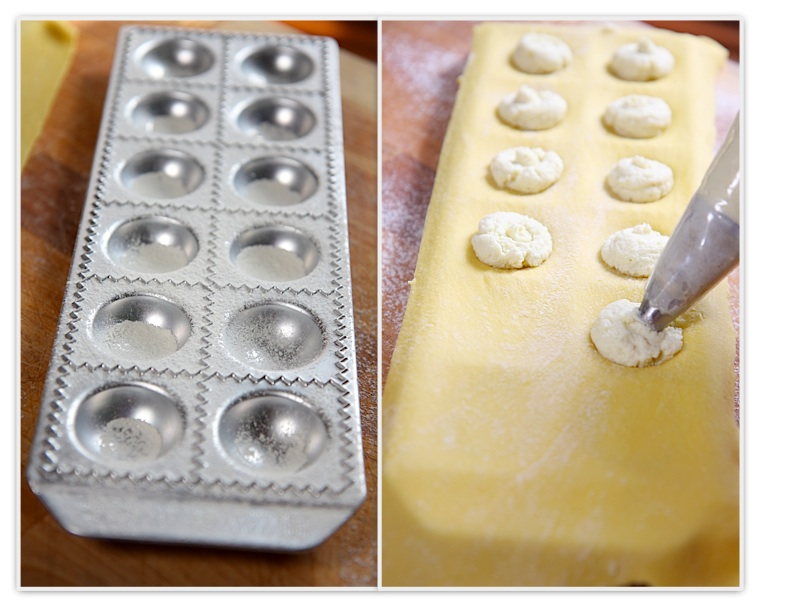
\includegraphics[scale=0.5]{images/raviolimoldwithfilling.jpg}
	 		 				\caption{Raviolimaskin}
	 		 				\label{ravioli}	
	 		 			\end{center}
	 		 		\end{figure}
Den andra typen av maskinen är väldigt stor med väldigt högt pris, som medför att de inte kan användas av hushåll, se figur 3.
 		\begin{figure}[h]
 			\begin{center}
 				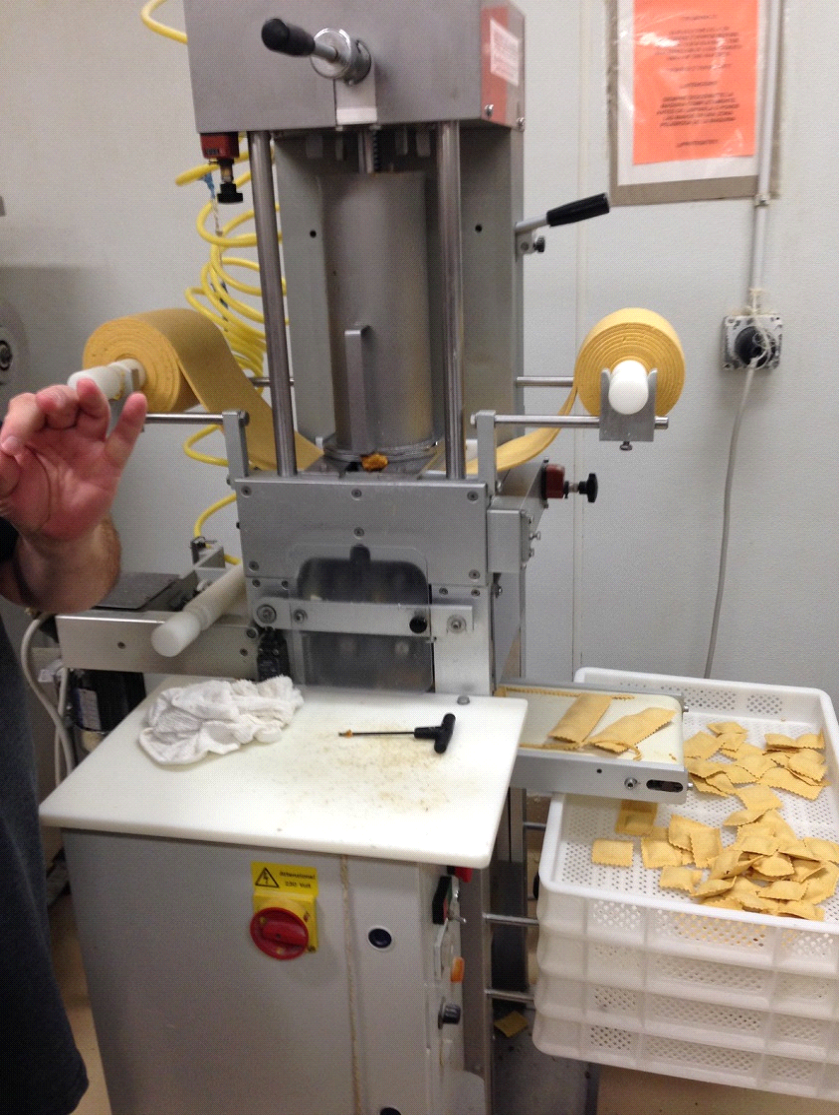
\includegraphics[scale=0.5]{images/ravioli_maskin.png}
 				\caption{Industriell Pasta/Raviolimaskin}
 				\label{pastamaskin}	
 			\end{center}
 		\end{figure}
		

Det finns olika typer av Ravioli maskiner på marknad redan nu. Entyp ravioli maskin som visas på figuren ?? är den enklaste modellen som underlättar lite processen, men det mesta görs manuelt. )
Detta projekt  ämnat till att skapa en Ravioli maskin. Projektet är en egen ide som skall utföras av två studenter vid Högskolan i halmstad.\\ 


Iden bakom projektet baseras på behov av en Ravioli maskin hemma.
Det finns färdiga industriella maskiner i marknaden. Dessa maskiner är väldig stora och tunga samt att de är dyra. 
Tanken är att man skapar en liten och biligt Ravioli maskin.		